\documentclass[10pt, journal,onecolumn]{IEEEtran}
\usepackage{cite}
\usepackage{graphicx}
\graphicspath{{figure/}}
\usepackage{array}
\usepackage{subfigure}
\usepackage{stfloats}
\usepackage{url}
\usepackage{nicefrac}
\usepackage{amssymb}
\usepackage{amsmath}
\usepackage{amsfonts}
\usepackage{amssymb}
\usepackage{booktabs}
\usepackage{relsize}
\usepackage[pdfpagelabels]{hyperref}
\usepackage{float}
\usepackage[round]{natbib}
\usepackage{color}
\usepackage{authblk}
\usepackage{caption}
\usepackage{enumerate}

\newcommand{\ra}[1]{\renewcommand{\arraystretch}{#1}}


% Allow paragraph indents inside lists.
%\usepackage{enumitem}
%\setenumerate{listparindent=\parindent}

%\usepackage{kbordermatrix}

\hypersetup{
  colorlinks   = true, %Colours links instead of ugly boxes
  urlcolor     = blue, %Colour for external hyperlinks
  linkcolor    = red, %Colour of internal links
  citecolor   = red %Colour of citations
}

\floatstyle{ruled}
\newfloat{algorithm}{tbp}{loa}
\floatname{algorithm}{Algorithm}

\newtheorem{theorem}{Theorem}
\newtheorem{corollary}{Corollary}
\newtheorem{proposition}{Proposition}
\newtheorem{definition}{Definition}
\newtheorem{lemma}{Lemma}

\newcommand{\norm}[1]{\left\lVert#1\right\rVert}
\newcommand{\abs}[1]{\left\lvert#1\right\rvert}
\newcommand{\inner}[1]{\left\langle#1\right\rangle}
\def\b#1{\mathbf{#1}}
\def\t#1{\text{#1}}


\title{Predicting the 2014 Ebola Outbreak in West Africa using Network Analysis \\
       {\large Final Report} }

\author{Shafi Bashar, Mike Percy, Romit  Singhai}
\affil{\textit {\{shafiab, mp81, romit\}@stanford.edu}}

\renewcommand\Authands{ and }


\begin{document}

\maketitle

\begin{abstract}
The current Ebola outbreak in West Africa is the worst in history.
Most traditional epidemiological models are compartmental models that have a random-mixing
assumption, calculating the effective reproductive rate of an outbreak.
We survey three of these models: the classic
SIR (Susceptible, Infectious, Recovered) model and two extensions used in Ebola research.

Network models allow for avoiding the random-mixing
assumption inherent in compartmental models.
This is done by assigning each individual a finite set of permanent contacts.
We review generated contact network models for SARS, including an urban network, a random network, and
a scale-free network.
We then propose a worldwide network model that takes an alternate approach to modeling
the flow of people based on economic trade data and attempt to predict the future
of the Ebola outbreak.

\end{abstract}



%%%%%%%%%%%%%%%%%%%%%%%%%%%%%%%%%%%%%%%%%%%%%%%%%%%%%%%%%%%%

\section{Introduction/Motivation/Problem Definition (15\%)}
\label{sec:Introduction}

In this paper we explore predicting an Ebola outbreak using a worldwide network of trading countries.



%%%%%%%%%%%%%%%%%%%%%%%%%%%%%%%%%%%%%%%%%%%%%%%%%%%%%%%%%%%%

%(10\%) of marks
\section{Related Work}
\label{sec:RelatedWork}

\subsection{\textbf{Compartmental Epidemiological model}}
\label{SubSec:SIR}

The majority of research in epidemiological theory is based on the compartmental model. To model the progress of an epidemic in a large population, the individuals in the population are compartmentalized according to the state of the disease. The most widely used such model is the SIR model introduced in \citep{very_old_paper}:

\begin{itemize}
\item \textbf{S (Susceptible):} Individuals who have not yet caught the disease from contact with an infectious
  individual.
\item \textbf{I (Infectious):} Individuals who have the disease. They have some probability of
  infecting susceptible people.
\item \textbf{R (Recovered):} Individuals who have experienced the full infectious period, and are
  now non-infectious and immune.
\end{itemize}

The changes among these states over time are represented by a set of differential equations. In
order to capture the dynamics of disease spread over time, a population-wide random mixing model is
assumed, meaning that each individual has a small and equal chance of coming into contact with
any other individual in the population. The basic reproductive number $R_0$
is defined as the average number of secondary cases generated by a primary case in a pool of mostly
susceptible individuals, and is an estimate of epidemic growth at the start of an outbreak if
everyone is susceptible. Almost all existing literatures \citep{chowell2004basic,legrand2007understanding,gomes2014assessing} on Ebola epidemic prediction are based on the modification of the basic SIR model.

In \citep{chowell2004basic}, the authors model the effect of Ebola outbreaks in 1995 in Congo and in
2000 in Uganda using a compartmental model similar to the SIR model in Section \ref{SubSec:SIR}. However, a
distinct feature of Ebola is that individuals exposed to the virus who become infectious do so
after a mean incubation period. In order to reflect this feature, in the SIR model is extended with
an additional ``Exposed'' compartment state. This SEIR model is reproduced in
Figure \ref{fig:SEIR_model}:

\begin{figure}[h!]
\captionsetup{justification=centering}
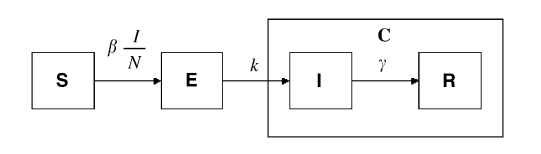
\includegraphics[scale=0.4]{seir_model_fig}
\centering\caption{SEIR model}
\label{fig:SEIR_model}
\end{figure}

In the SEIR model, susceptible (S) individuals in contact with the virus enter the exposed (E) state
at a rate of $\beta I / N$.
The exposed (E) individuals undergo an average incubation period of $1/k$ days before progressing to
the infectious (I) state. The exposed state is assumed to be asymptomatic as well as uninfectious.
Infectious (I) individuals move to the R state, either recovered or dead, at a rate of $\gamma$.
 The parameters are $\beta$, the transmission rate per person per day;
$N$, the total effective population size; and $I/N$, the probability that contact is made with
an infectious individual.

In \citep{legrand2007understanding}, the Ebola outbreaks in Congo in 1995 and Uganda in 2000
are also studied. However, they expand on the model from \citep{chowell2004basic} by modeling the spreading of Ebola in heterogeneous settings. In order to gain more insight into the epidemic dynamics,
the infectious phase is subdivided into three stages: infection in a community setting (I), infection in a hospital setting (H), and infection after death assuming a traditional funeral (F). The resulting model is known
as the SEIHFR model. 

A CDC (Centers for Disease Control and Prevention) report \citep{meltzer2014estimating} published in September 26, 2014 make use of the SEIHFR model to provide an estimate of the future number of cases of current Ebola epidemic. While SEIHFR model provides finer grained modeling of the behavior of Ebola, it is also complex and the link to a network-based model becomes tenuous. In addition, current 2014 Ebola epidemic is still in progress and we do not have the entire picture of the epidemic cycle. Given the limited number of data points, trying to fit a model will large number of parameters may lead to overfitting.  Because of these reasons, we do not plan to use the SEIHFR model in our work.

\subsection{\textbf{Network based Epidemiological model}}

In the compartmental models described in previous section, the underlying assumption is random mixing among population. Therefore, an infected individual can infect any other individuals in the population. Even though \citep{legrand2007understanding} modified the SEIR model to reflect the heterogeneity of infection states, the underlying assumption is still random mixing. However, contagious diseases like Ebola spread via networks formed by physical contacts among individuals. While an individual may have the same number of contacts per unit time in either a random mixing model or a network contact model, within a static network model the set of
contacts is fixed, versus a random-mixing model wherein it is continually changing. A static network model thus captures the permanence of many human relationships. 

In our search for existing literature on networks based model on spreading of Ebola, we haven't come across any previous work that precisely does this, possibly due to the lack of detailed data in the locations historically affected by the disease.  In \citep{newman2002spread}, the authors provide the relation between the compartmental SIR model and a random network model. The author introduces the concept of transmissibility in a network model. Transmissibility of a disease in a network model is defined as the average probability that an infectious individual will transmit the disease to a susceptible individual with whom they have contact. The authors also provide equations that connects the transmissibility and degree distribution of a random network with the basic reproductive number of an SIR model.  

In \citep{meyers2005network}, the authors model the spread of the 2002-2003 outbreak of SARS in Hong Kong and Canada using a network model. A contact network model attempts to characterize every interpersonal contact that can potentially lead to disease transmission in the
community. Each person in the community is represented as a node in the network and each contact between
two people is represented as an edge connecting them.
In \citep{meyers2005network}, the authors presented three different contact network models for SARS -  \textit{(a) Urban Network:} A plausible urban-setting contact network generated using simulation based on data from City of Vancouver, Canada. Households were randomly chosen and  their members given ages, schools, occupations, hospital beds as patients, and  caregivers according to statistics from public data.  This model offers a high degree of realism, but is complex. \textit{(b) Random Network:} A random network with Poisson degree distribution in which individuals connect to others independently and uniformly at random. \textit{(c) Scale-free Network:}  A truncated power law degree distributed network can model individuals, called ``superspreaders'' with unusually large numbers of contacts or ``supershedders" who are unusually effective at
  excreting the virus into the environment they share with others. 
  
%Transmissibility $T$ of a disease in a network model is defined as the average probability that an infectious
%individual will transmit the disease to a susceptible individual with whom they have contact. The epidemic threshold $T_c$ is the minimum transmissibility required for an outbreak to become a large-scale epidemic.  In \citep{meyers2005network}, authors extended the results from \citep{newman2002spread} to provide the relations between the basic reproductive number
%$R_0$ of an SIR network and the transmissibility $T$ and epidemic threshold $T_c$ of a random networks.
% as follows:
%
%\begin{equation}
%R_0 = T  \dfrac{\left\langle k^2 \right\rangle}{\left\langle k \right\rangle-1},
%\quad\quad
%T_c =\dfrac{\left\langle k \right\rangle}{\left\langle k^2 \right\rangle - \left\langle k \right\rangle}
%\end{equation}
%
%where, $\left\langle k \right\rangle$ and $\left\langle k^2 \right\rangle$ are the mean degree and
%mean square degree of the network.
%
Neither \citep{meyers2005network, newman2002spread} captured the temporal progression of the epidemic using network model. Instead, the authors provide the final number of infected nodes in a network for a given value of $T$. Compare to the compartmental model, there are two major drawbacks in the network based model 

\begin{enumerate}[(a)]
\item Compartmental model is well-established model and can generally capture the temporal progression of disease spread in a localized population fairly well. In contrast, with a contact  network, it is hard to model the spread of disease over time. In general, percolation theory is used in conjunction with a contact network to predict the final number of individuals that can get affected in a given network. However, it is generally hard to  predict the stage of the disease at a given time with a network model. 

\item In general, it is almost impossible to model the actual contacts among individuals. Therefore, in most network model, additional assumptions are made to model the contact network.
\end{enumerate}

\subsection{\textbf{Combination of Compartmental and Network based Epidemiological model}}

As discussed in previous sections, a compartmental model is convenient in analyzing the temporal progression of a contagious disease in a localized population. However, due to the underlying assumption of random mixing among populations, such model is not suitable to analyze large scale outbreak of contagious diseases in a world-wide scale. A much attractive alternative solution in analyzing the progression of disease in a world-wide scale is a combination of compartmental and network model. In such formulation, compartmental model is used on a local scale to track the progression of disease in individual countries (cities or continents). To capture the dynamics of inter-country (city or continent) spread of disease, some form of network data can be used. Such network data are usually converted to inter-country (city or continent) transfer of population per unit time.

In \citep{balcan2010modeling} the authors model the inter-country and inter-city spread of population using airport network data and commuting network data. The authors then use such model in conjunction of stochastic compartmental model to analyze the  2001-2002 seasonal influenza spreading. A similar works  \citep{gomes2014assessing}  attempts to predict the spread of Ebola to different parts of the world based on a model that incorporates both the compartmental approach and the use of world-wide air traffic flows. In this model, the world is divided into geographcal regions defining a subpopulation network, modeling connections among subpopulations representing traffic flows due to transportation infrastructure.

\bigskip




%%%%%%%%%%%%%%%%%%%%%%%%%%%%%%%%%%%%%%%%%%%%%%%%%%%%%%%%%%%%

%   Model/Algorithm/Method (30%) + Results and findings (35%)

\section{Modeling localized epidemic spread using a random mixing model}
\label{sec:IntraCountry}

In first phase of the project, to calculate the basic reproductive number of the current Ebola
epidemic spread in different countries, we performed model fitting on the data we gathered from
\cite{cmriversdata}. We considered the SEIR model described in \cite{chowell2004basic}. The following set of differential equations are used to represent this model \cite{chowell2004basic}:

\begin{equation}
\dfrac{dS}{dt}	=	\dfrac{-\beta SI}{N},
\quad
\dfrac{dE}{dt}	=	\dfrac{\beta SI}{N}-kE,
\quad
\dfrac{dI}{dt}	=	kE-\gamma I,
\quad
\dfrac{dR}{dt}	=	\gamma I,
\quad
\dfrac{dC}{dt}	=	kE.
\label{Eq:SEIR}
\end{equation}

Here, $S$, $E$, $I$, and $R$ denote the number of susceptible, exposed, infectious and removed
individuals at time $t$. $C$ is not an epidemiological state, however it is useful to keep track of the cumulative
number of infected cases from the time of the onset of the outbreak. In order to model the effect of intervention on the spread of the disease, in the above model, the transmission rate $\beta$ is modeled as a function of time. At the initial phase of the outbreak, before intervention, $\beta$ is parameterized by $\beta_0$. After intervention, the value of $\beta$ transitions from $\beta_0$ to $\beta_1$, $\beta_0>\beta_1$ as follows:

\begin{equation}
\beta(t)=\begin{cases}
\beta_{0} & t<\tau\\
\beta_{1}+(\beta_{0}-\beta_{1})\exp\left(-q\left(t-\tau\right)\right) & t\ge\tau
\end{cases}
\label{Eq:Beta}
\end{equation}

Where $\tau$ is the time when interventions begin and $q$ controls how quickly the rate
of transmission changes from $\beta_0$ to $\beta_1$.
The SEIR model under consideration is a non-linear model with six parameters. The current Ebola epidemic is
still spreading and depending on the preventative measures  taken, the underlying dynamics of the
spread can change drastically any time. The Ebola data for three most affected countries in West Africa - Guinea, Sierra Leone and Libera were represented as $(t_i,y_i)$, $i=1,2,\ldots,n$ where $t_i$ represents $i$th reporting time and $y_i$ the cumulative number of infectious cases from the beginning of the outbreak of to time $t_i$.  The model parameters $\Theta=(\beta_0,\beta_1,k,q,\gamma, \tau)$ for these three countries were estimated using a non-linear least-square procedure by fitting these data to the cumulative number of cases $C(t,\Theta)$ in Equations \ref{Eq:SEIR},\ref{Eq:Beta}. In addition, we performed model fitting for the West Africa region
by adding up the data from these three countries. 

Given the limited number of data available, instead of fitting all six parameters to the model, we decided to fix some of the parameters based on studies on previous Ebola epidemics. In \cite{chowell2004basic}, the incubation time of the Ebola virus $1/k$ is found to vary between 1 and 21 days, with a mean time of 6.3 days for previous Ebola outbreaks. For ease of data fitting, we set this parameter value to the mean value of 6.3 days.
We note that the dynamics of the current epidemic may differ from previous ones, and therefore
fixing a value based on the prior estimate may lead to some inaccuracy.  The choice of selecting initial outbreak time $t_0$ and intervention time $\tau$ is a difficult problem. To this end, we looked into different sources like WHO (World Health Organization) and CDC websites to learn more about the timeline of the spread. In Guinea, a 2-year-old boy died on December 2, 2013, later diagnosed as an Ebola patient. We consider this
incident as the index case for Guinea and set $t_0$ to December 2. On March 2, the Government of
Guinea informed WHO regarding the possibility of an Ebola epidemic and declared a national heath
emergency. We considered this date as the intervention date and set $\tau$ to 110. In Sierra Leone,
one person died on April 2014. In June 12, 2014 the country declared an emergency and closed its borders
with neighboring Guinea and Liberia. We consider the first date as $t_0$ and second date as the
intervention time, therefore set $\tau$ to 50. In Liberia, on March 31, 2014, there was official
confirmation of two people infected with Ebola. We set this date to $t_0$ and set $I_0$ and
$C_0$ in our model as 2. The government of Liberia shut down all schools on July 30, 2014. We
consider this date as the date of intervention in Liberia and set $\tau$ to 120.

%In order to fit the non-linear SEIR model to the data, we used non-linear least squares estimation. We
%use the reported data $(t_i, c_i)$ for $i=1,2,\ldots,n$ where $t_i$ denotes the $i-th$ reporting time
%and $c_i$ the cumulative number of infectious cases from the beginning of the outbreak at time $t_0$ to
%time $t_i$.
The optimization problem involving the model fitting of SEIR model is a non-linear least square regression problem and contains a large number of local minima. Therefore, the choice of initial parameter estimate is an important consideration to get the globally optimal solution. In order to find a good initial choice of the parameters as input to the non-linear least squares solver, we first perform a Latin hypercube sampling on the  4-dimensional parameter space.  We grid up the hypercube with a number of grid points in each dimension.  We then choose the sample that minimizes the least squares error as the initial input. In order to calculate the 95\% confidence
interval of the estimated parameter, we performed bootstrapping based on residual error.

\begin{figure}[ht]
\centering
\subfigure[Guinea]{
  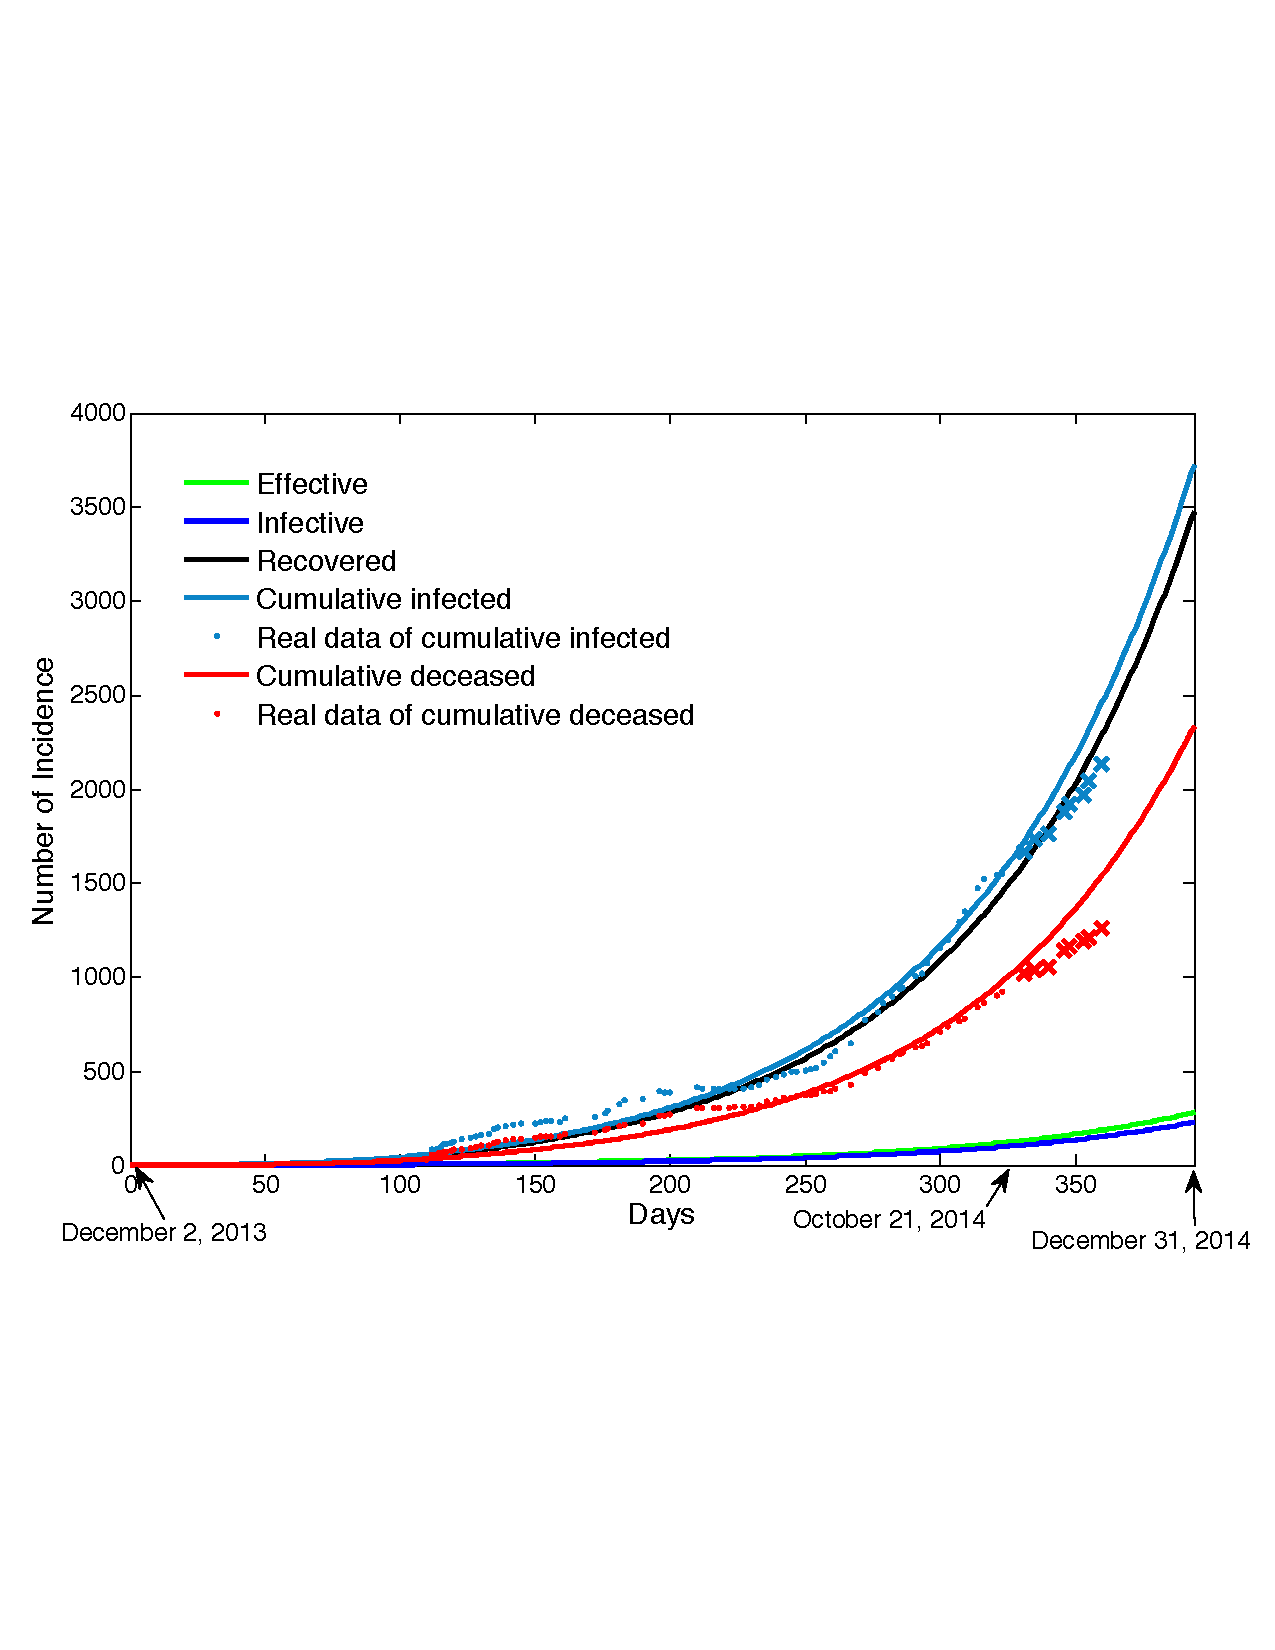
\includegraphics[width=0.45\textwidth]{Guinea1.pdf}
  \label{fig:subfigure1}}
\quad
\subfigure[Sierra Leone]{
  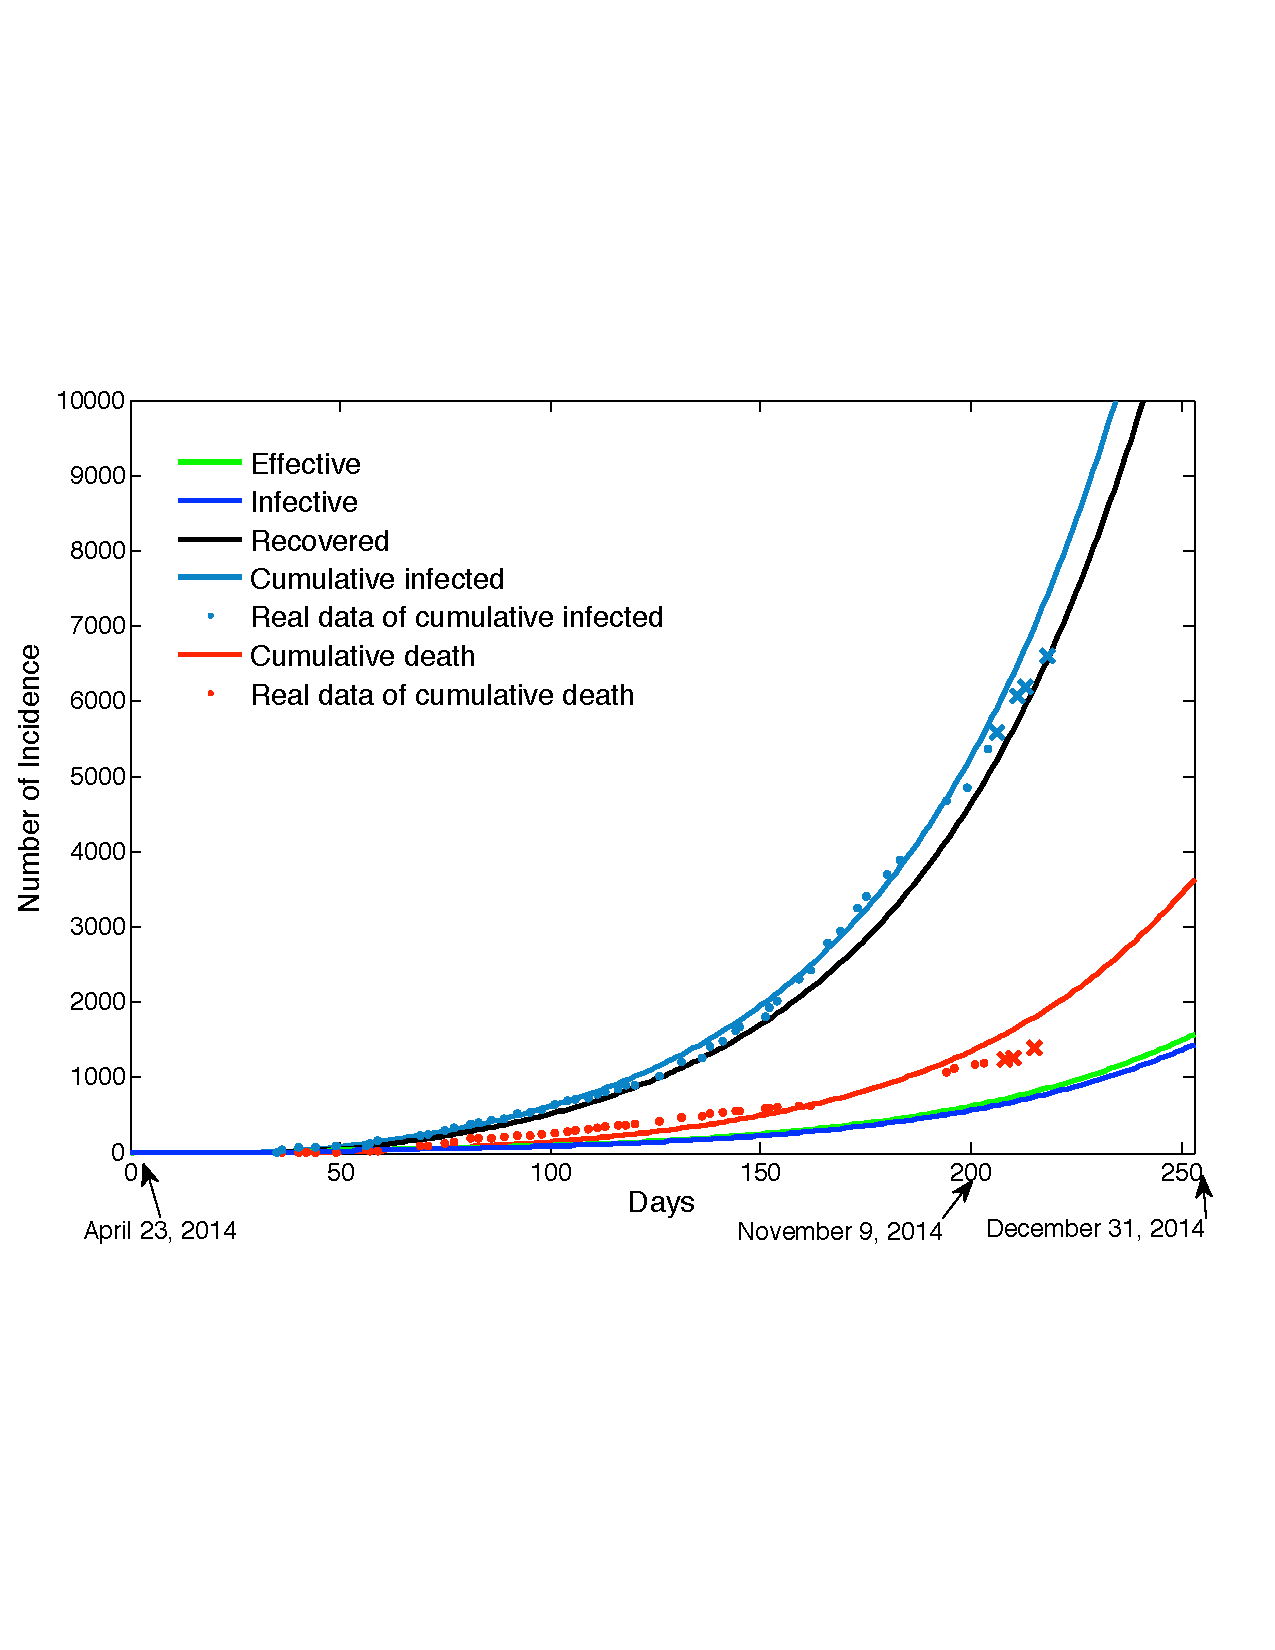
\includegraphics[width=0.45\textwidth]{SierraLeon1.pdf}
  \label{fig:subfigure2}}
\subfigure[Liberia]{
  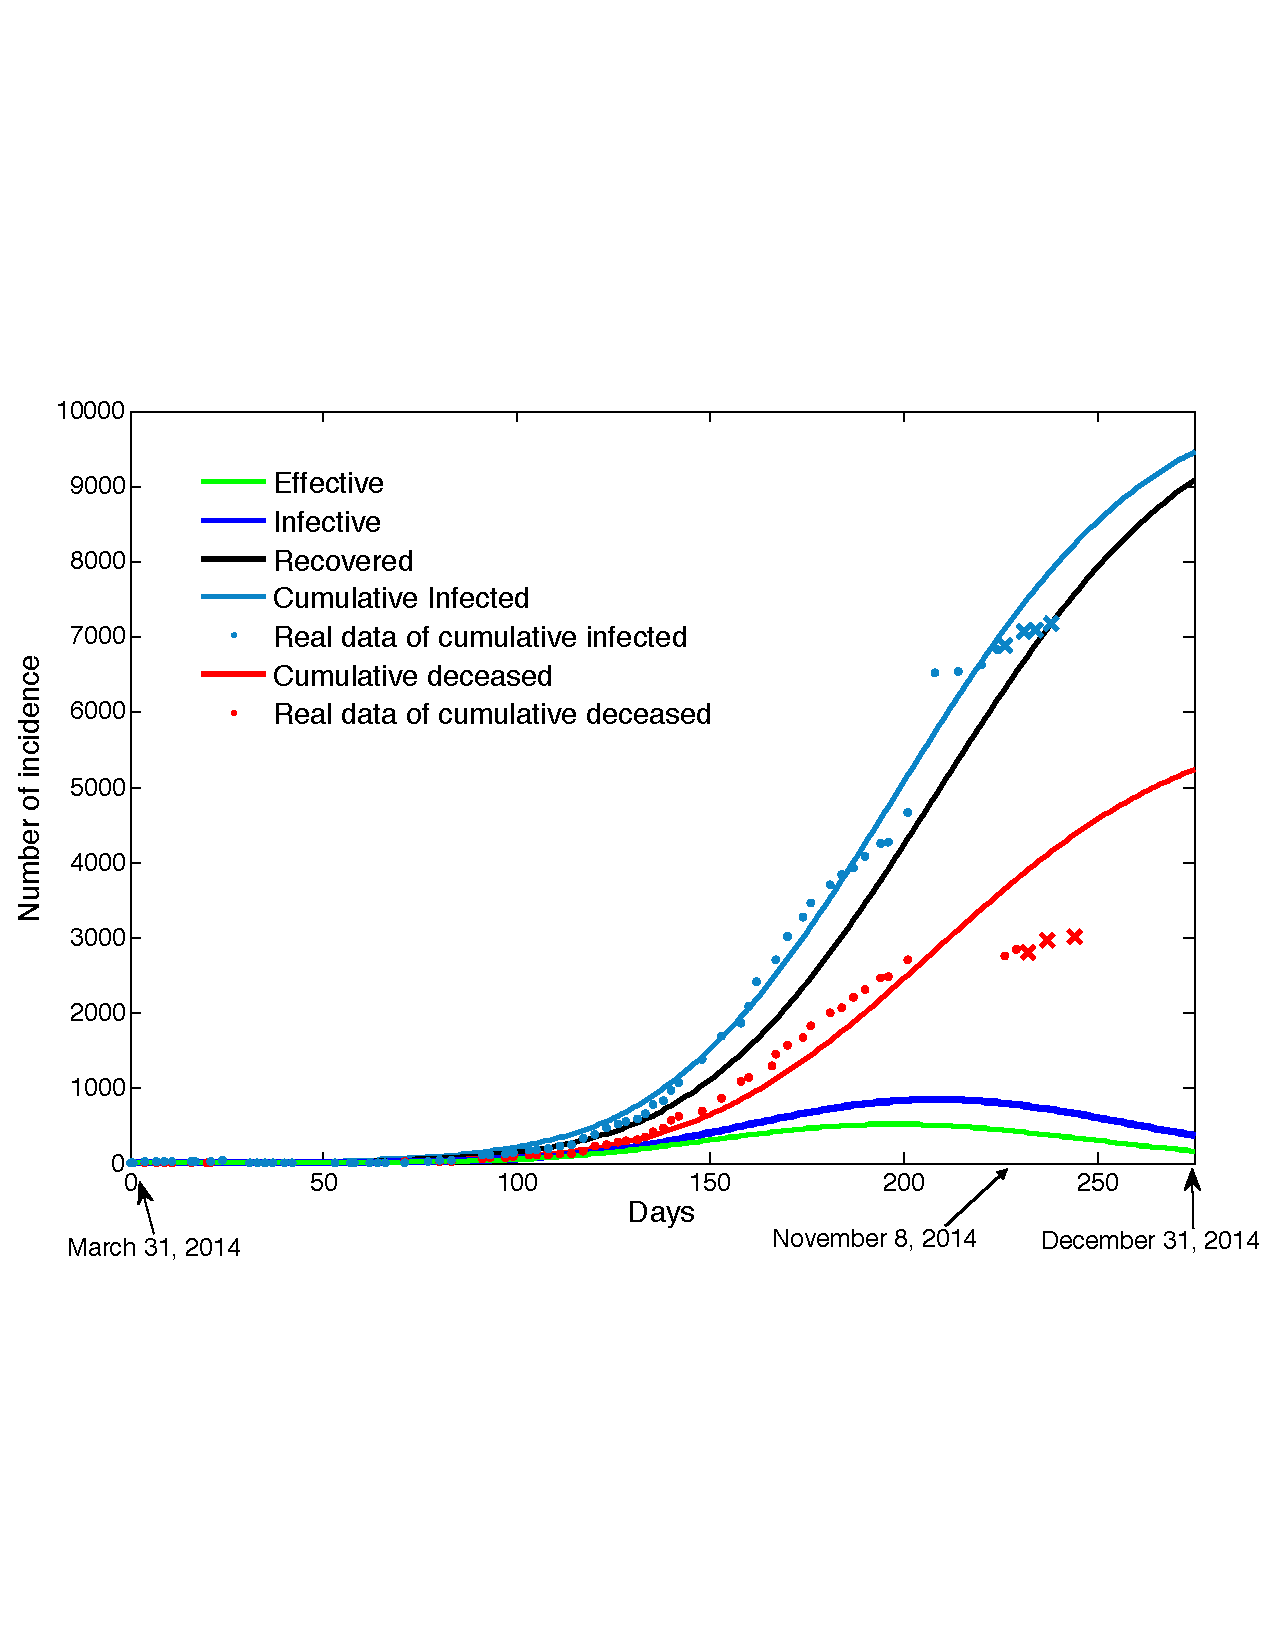
\includegraphics[width=0.45\textwidth]{Liberia1.pdf}
  \label{fig:subfigure3}}
\quad
\subfigure[West Africa]{
  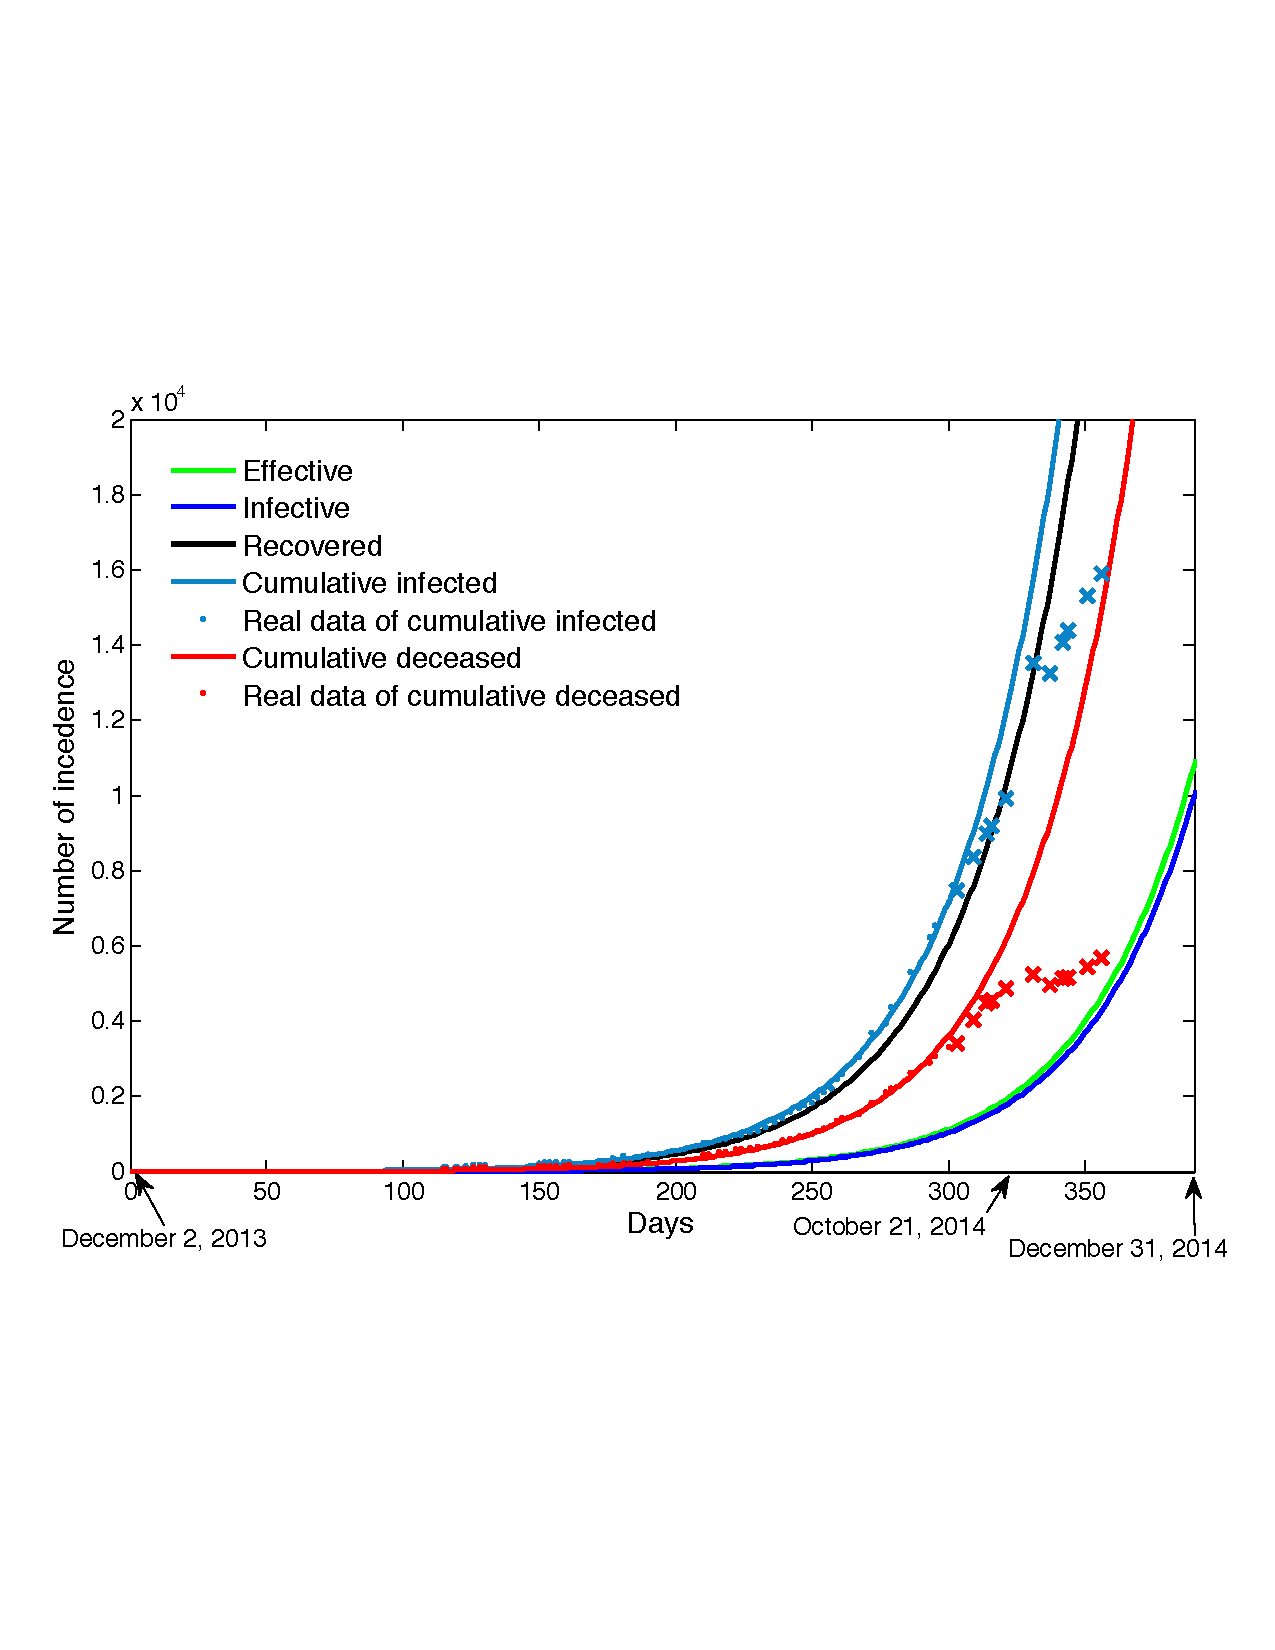
\includegraphics[width=0.45\textwidth]{WestAfrica1.pdf}
  \label{fig:subfigure4}}

\caption{SEIR model fit results for 2014 Ebola epidemic data}
\label{Fig:figurePrediction}
\end{figure}


The estimated parameters for the SEIR model of Guinea, Sierra Leone, Liberia, and the overall West Africa 
region is presented in the Appendix. In Figure \ref{Fig:figurePrediction}, we presented the number of incidents at different compartments of the SEIR model, as well as the cumulative number of infectious cases over time. In our project milestone report, our model fit was based on the last data we collected on Oct. 21, 2014. At the time of writing this final report, we have additional data points available. Based on data collected till November 9, 2014, we have updated our parameter estimation for Sierra Leone and Liberia. We, however, kept the same model for Guinea as in our milestone report, since we have the most amount of data available for Guinea already due to an earlier outbreak date in Guinea (Dec. 2, 2013). We extrapolated the graph up to Dec. 31, 2014.  We note that forecasting future cases may not be accurate as the underlying factors of the epidemic are changing rapidly with the increase in safety measures. The unused data for Guinea (Oct. 21 - Dec. 5), Sierra Leone (Nov. 10 - Dec. 5) and Liberia (Nov. 10 - Dec. 5) are used for calculating test error. These values are also plotted in Figure \ref{Fig:figurePrediction} (points represented with `.' sign are used for training, points represented with `x' sign are used for testing). We observe that the predictions of the model to the cases up to Dec. 5 are mostly on par with the observed data for Guinea, Sierra Leone and Liberia. For the Guinea epidemic, we have data for the longest range of days and the estimated model, therefore, captures most of the
dynamics of the spread in contrast to the other cases.  

For the West Africa region plot, our prediction number is much higher than the actual data. This is understandable, as the underlying assumption behind the SEIR model is random mixing.  Within a country without any movement restriction, this model is somewhat appropriate. However, for the aggregated model among multiple countries, this assumption is no longer valid due to stricter movement regulations between country borders. Therefore, a model with a random mixing assumption will overestimate the number of infectious cases.


\begin{table}[h]
\caption{Estimated number of total infected people (by December 31, 2014) and root mean square error (RMSE) of prediction} 
\centering
\begin{tabular}{|c|c|c|c|}
\hline 
Country & Estimated Number of Infected individuals & Cross-validation Error & Test Error 
\tabularnewline
\hline 
\hline 
Guinea & 3724 & 100.96 & 218.9\tabularnewline
\hline 
Sierra Leone & 14040 & 170.14 & 546.2\tabularnewline
\hline 
Liberia & 9500 & 350.3 & 504.24\tabularnewline
\hline 
\end{tabular}
\label{Tb:prediction}

\end{table}

In Table \ref{Tb:prediction}, we presented our estimate of the total number of people who could get infected by December 31, 2014 as well as root mean square cross-validation error of our model fit and test error on the unused data. 

%As an extension of the above approach, for finding parameters for the model based on the current data,
%we designed and ran a simulation using an MCMC approach with input as time series data for the
%various infected regions. Initial values for the various parameters were assumed as above for the
%prior distribution, but a range based on the literature was used to find the most appropriate
%values for the current outbreak. For example $\beta_0$  had a range of $[0,1]$,  $\beta_1$ had a range of
%$[0,1]$, infection time $1/\gamma$ had a range of $[3.5,10.7]$, incubation time $1/k$ had a range of $[5,22]$,
%and $\tau$ had a range of $[100,150]$. This simulation is running and we will
%have results in the final report.




\section{Mapping the compartmental model to the network based model}




\subsection*{\textbf{Problem Definition}}
Since the compartmental models used in predicting spread of epidemics have a random mixing assumption which may not model the real world appropriately. In this section we made an attempt  to map the compartmental model to network based model  using percolation theory to study  and model the spread of Ebola in West Africa.

\subsection*{\textbf{Approach}}

The mapping between a compartment mode and a network based model is defined in the paper by \cite{meyers2005network}.The transmissibility $T$ of a disease which is defined as the average probability that an infectious
individual will transmit the disease to an individual with whom they have contact. 
We start with the reproductive number $R_0$ calculated using the compartmental model.
Using the relationship between the basic reproductive number
$R_0$ and the transmissibility $T$  defined by Meyers as:

\[
R_0 = T  \dfrac{\left\langle k^2 \right\rangle}{\left\langle k \right\rangle-1}
\]

We calculate the transmissibility.

We also calculate the value of epidemic threshold $T_c$, which is defined by Meyers as:

\[
T_c =\dfrac{\left\langle k \right\rangle}{\left\langle k^2 \right\rangle - \left\langle k \right\rangle}
\]

We use these numbers in modeling and analysis of our contact networks.


\subsection*{\textbf{Data Preparation}}

For simulating a contact network for Ebola in various infected countries we used a data set from a social networking site available on
the \cite{topcoderdata}.
This undirected network has 4,846,609 nodes and 42,851,237 edges and average degree of $8.841$.
It is clearly a scale-free network because the degree distribution follows a power law after a degree of
approximately 50.

We calculated the transmissibility values for each of the countries Liberia, Guinea and Sierra Leone in West Africa  using the formula described above. 

\begin{center}
    \begin{tabular}{ | l | l | l | p{5cm} |}
    \hline
    Country & $R_0$ & Transmissibility \\ \hline
    Liberia & 0.001 & 0.001  \\ \hline
    Guinea & 1.145 & 0.1148 \\ \hline
    Sierra Leone & 1.24 & 0.1243  \\ \hline
    \end{tabular}
\end{center}

We also generated three other datasets  for a preferential attachment network, random network and a small world network approximating the real network for comparison purposes.

We calculated the epidemic threshold  $T_c=0.1275$  using k=8.841 and the formula described above.

These values will be used for running the simulation on the various network datasets.

\subsection*{\textbf{Simulation}}

Since our datasets were  large and simulation using a percolation model is a compute intensive process so it was not possible to run the simulations in the reasonable time on a local machine.

We ran our simulations on  extra large EC2 instance (c3.8xlarge). Since our simulations needed to run for multiple values  of Transmissibility we developed a test harness to  run the simulations  model written in  python in parallel using 

http://www.gnu.org/software/parallel/ to leverage  multiple  cores of the EC2 instance.  Our simulation using  all four datasets and 20 different values of T  completed in  about 7 hrs for 200 iterations.


\subsection*{\textbf{Results and Conclusion}}

\begin{figure}[ht]
\centering
\subfigure[Network Simulation for Ebola]{
  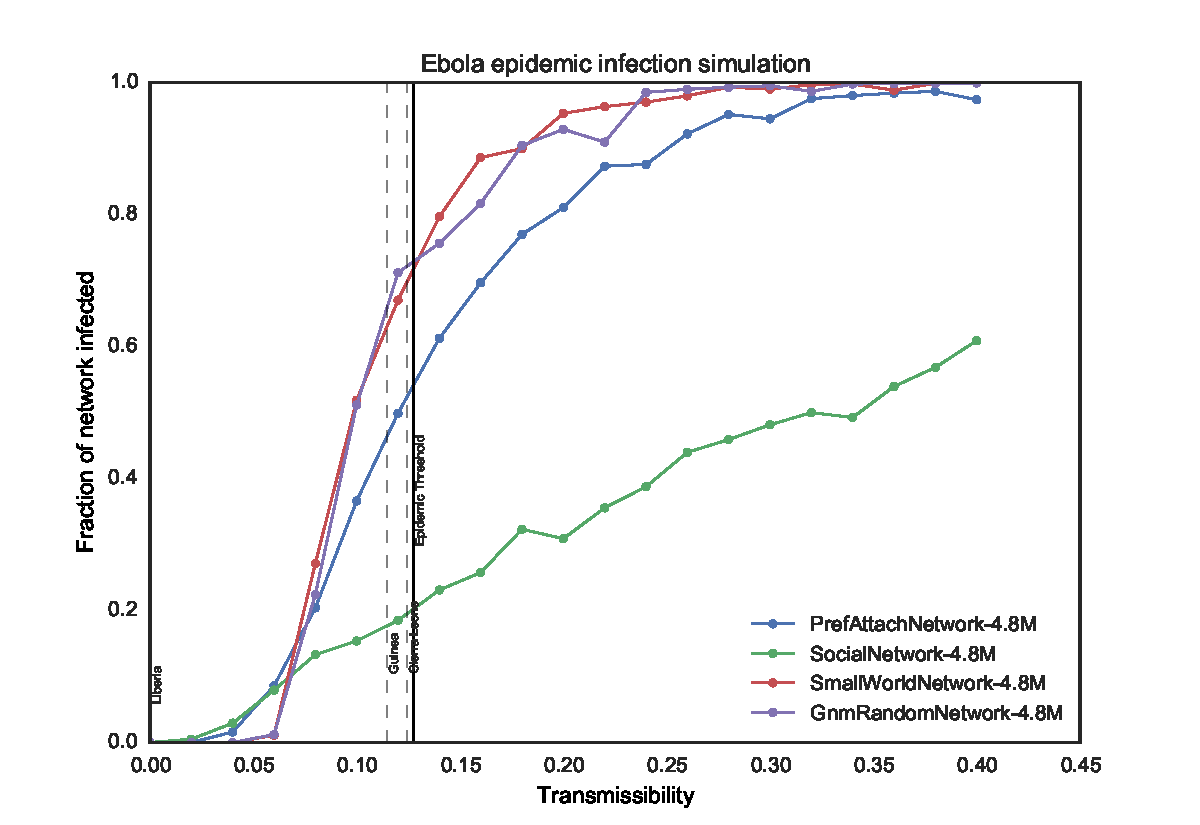
\includegraphics[height=0.8\textwidth]{EbolaNetworkSpread.pdf}
  \label{fig:Network Simulation for Ebola}}
\end{figure}


Above figure show the percentage of network infected for different values of Transmissibility for  various network types.  The real world network has a constant slope for  increasing value of Transmissibility even beyond Epidemic Threshold and higher values of transmissibility in comparison to other network types.
It is followed by a synthetic preferential attachment network following a perfect power law distribution. For Preferential attachment, Small World and Random Networks for value of T in the range of 0.35-0.40 [R in range 3.5-4] nearly the entire network gets infected but not for real network.

\subsection*{\textbf{Future Work}}

Since the countries  severely impacted by Ebola are not technically  advanced  it will be  very interesting to infer the hidden network using the cascade diffusion model. Running simulations on  the inferred network and comparing  with the actual results can provide better insights into the spread of  current epidemic. The transmission probabilities and other heuristics developed can be used in future.

\subsection*{\textbf{Contribution}}




\section{Predicting worldwide spread}
\label{sec:Worldwide}

\subsection*{\textbf{Approach}}
In order to simulate how the Ebola epidemic might spread across the world, we have assembled a
worldwide network based on international trade. Because the trade numbers are in US dollars,
we have assumed a linear relationship between exports in dollars and travelers going abroad.
This is a strong assumption, and we are considering more sophisticated mappings.
We are using this as a long-range network representing trade-based population movement and
connecting localized subnetworks with these trade-driven edges. We are developing a simulation
framework to run in discrete time steps and predict the spread of Ebola across this worldwide network.

\subsection*{\textbf{Trade network data preparation}}

The trade network dataset we are using is based on data retrieved from the web service API to the
UN Comtrade database \citep{uncomtradedata} via their web service API.
The data queried for were country-to-country SITC-1 exports from the latest data available
for each country.

Several problems with this raw dataset immediately became apparent which required working around.
Many war-torn countries such as Liberia have not reported detailed export data
to the UN in decades (Liberia last reported in 1984). As a result of this, the export totals
are incorrect for the present day. In addition, this old data reports exports to countries that
no longer exist, including East Germany and Yugoslavia. In order to make the dataset usable for
modern-day predictions, we performed the following transformations on the data (using Perl scripts):

\begin{itemize}
\item Manually remapped non-existent countries to their modern equivalents.
      In a few cases, we had to do a best-effort mapping. For example, Yugoslavia split into many
      states, so we assign exports to historical Yugoslavia to modern-day Slovakia,
      since Slovakia currently has the largest economy of the states that once comprised Yugoslavia.
\item Removed exports from states that no longer exist, preferring export data from
      modern equivalents.
\end{itemize}

We then needed to make the per-country exports sum up to the latest available export data.
The United States \cite{ciatotalexports} World Factbook contains up-to-date export totals
for most countries in the world. Using the above data set, on the (admittedly strong) assumption
that the export distribution
from country-to-country in the UN Comtrade data set has remained the same between the last year a
country has reported detailed export data and the latest totals from the CIA, we linearly renormalized
each outgoing edge in our data set so that the total sum of exports equalled the latest CIA data
for each country.
This required a manual step of mapping country names in the UN dataset to those used in
the CIA dataset.

Once we had a ``renormalized'' dataset including detailed export edges and totals matching
the latest available data, we needed to map these numbers to theoretical international travelers.
We could not find complete, or even nearly complete, publicly available data on the number of
international outgoing travelers per country. While inbound tourism numbers are available from
\cite{worldbankinboundtourism}, for the outbound tourism numbers from \cite{worldbankoutboundtourism},
many countries are missing,
especially the African nations that we care so much about from an Ebola outbreak perspective.
Some data are available from the \cite{unwtooutboundtourism}, however they appear to be behind a paywall.
Data for total air travellers are available from \cite{worldbankairpassengers},
however this total includes domestic flights and so is less useful for our purposes.

Our current approach to map outbound dollars to outbound travelers is to assume a linear relationship
between these numbers, and also to assume that the same linear relationship holds for imports to
inbound tourists to a country.
We currently use the United States as a model and use the ratio of
imports to the United States per year to the number of tourists visiting the United States per year.
Based on data from the \cite{usinboundtourists}, 69.77 million people visited the United States in 2013.
According to our renormalized data set, total imports into the United States were
\$$2.21$ trillion during the same period. Dividing imports by visitors (an admittedly
simplistic approach) gives us a scaling factor of approx. $31,665$. Therefore we have applied this
scaling factor to all edges in our international exports network, giving us some approximation of
outbound travellers from country to country based on export numbers.

\subsection*{\textbf{Supplementing the trade network}}

Using a trade network has its flaws, even discounting errors stemming from poor approximations.
For one, a trade-centric network ignores activity with low economic impact, such as
a vegetable farmer traveling to a nearby country to sell his products at the market, or someone
driving across the border to visit a family member. Relative to the economic impact of the industrial
diamond or rubber trade (exports of Liberia) for example, these potentially disease-spreading behaviors
simply are not represented equitably if at all in the model. On the other hand, economic trade data is
widely accessible and is likely to be fairly accurate,
and certainly it is safe to assume that that trade activity correlates with travel between two countries.

Due to the above drawbacks, we plan to supplement our trade network with a generated network that
captures local commute-related movement as well. One approach to generating such a network is the gravity law,
used for example to study traffic on Korean highways by \cite{jung2008gravity}. The gravity law
claims that the number of trips from point A to point B is inversely proportional to the square
of the distance between them.

\begin{figure}[ht]
\centering
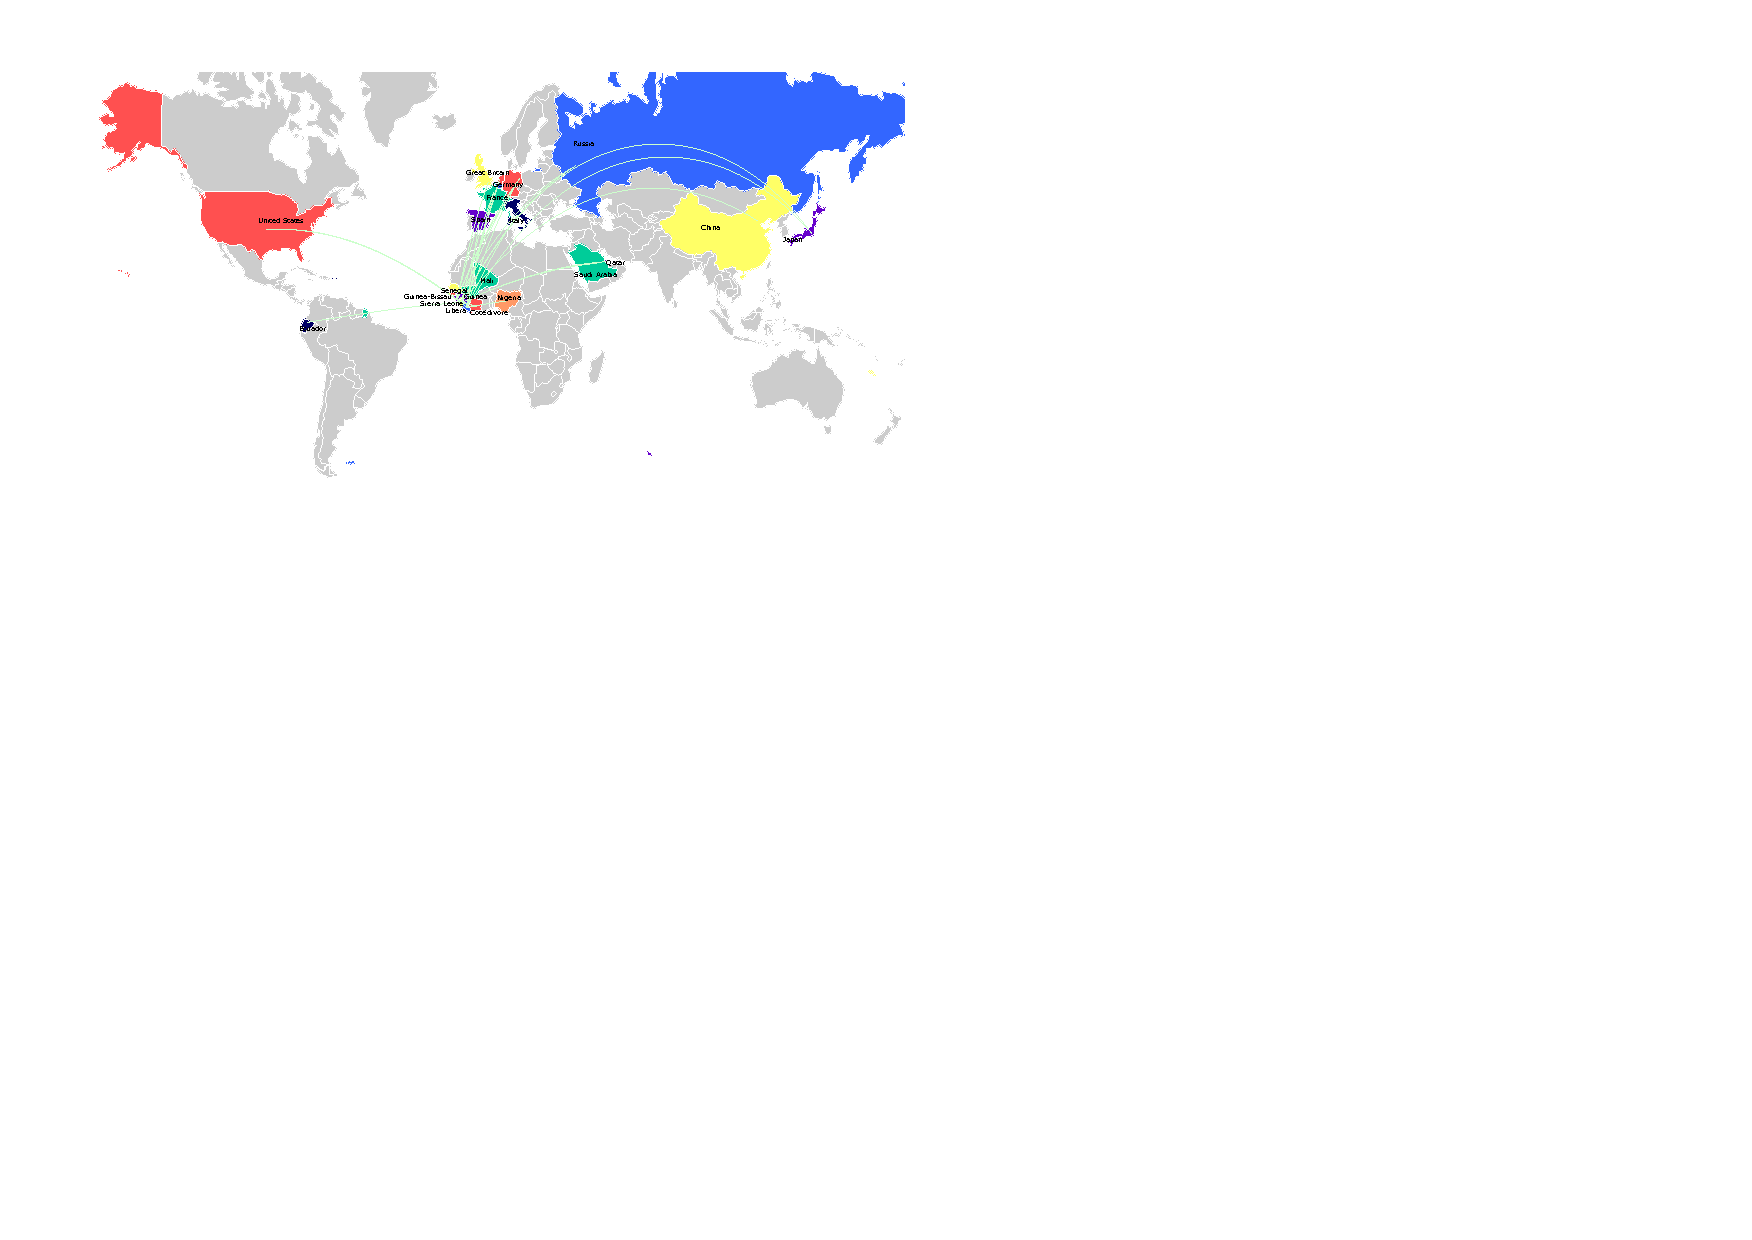
\includegraphics[scale=1.1]{world1.pdf}
\caption{World-wide trade network from Guinea, Sierra Leone and Liberia}
\label{Fig:worldtrade}
\end{figure}


\subsection*{\textbf{Simulation model}}

We are currently developing a simulation framework to incorporate intra-country spreading behavior
(using compartmental and network-based models) with inter-country links based on the above
worldwide network models. A related but distinct approach is the GLEaM stochastic simulation model
developed by \cite{balcan2010modeling}. Our simulation model is a stochastic, discrete time-step
model in which each time step is one day, and for each day, each infectious individual may travel
to another country with some probability related to the number of people leaving the country
via the worldwide networks on that day and the total population of the country. Within each country,
infectious individuals spread their disease with some probability related to the intra-country model
being used (compartmental or network-based).

\begin{figure}[ht]
\centering
\includegraphics[scale=.5]{countriesinfected.pdf}
\caption{Potential countries that could get infected and potential number of infected by December 31, 2014}
\label{Fig:worldtrade}
\end{figure}







%%%%%%%%%%%%%%%%%%%%%%%%%%%%%%%%%%%%%%%%%%%%%%%%%%%%%%%%%%%%

\bibliographystyle{plainnat}
\bibliography{bib_ref}



%%%%%%%%%%%%%%%%%%%%%%%%%%%%%%%%%%%%%%%%%%%%%%%%%%%%%%%%%%%%

\begin{appendix}


\begin{table*}[h]
\label{Table:parameter}
\caption{Parameter estimation for Ebola SEIR model (Guinea \& Sierra Leone)} 
%\hrule
\centering
\tiny
\parbox{.55\linewidth}{\centering
\ra{1.3}
\begin{tabular}{@{}crccc@{}}%\toprule
& \multicolumn{3}{c}{\textbf{Guinea}} &  \\
\cmidrule{2-4}
\textbf{Incidence Dependent Parameters} & \textit{Value} && \textit{Comments} \\
\midrule
Initial Case $t_0$ & December 2, 2013 &  & one person fell ill\\
$S_0$ & 0& & -\\
$E_0$ & 0& & -\\
$I_0$ & 1& & -\\
$R_0$ & 0& & -\\
$C_0$ & 1& &-\\
Intervention time & March 2, 2014 &  & Gov. of Guinea informed WHO\\
$\tau$ &110 & & -\\
\cmidrule{2-4}
\textbf{Estimated Parameters} & \textit{Value} & \textit{95\% CI} & \textit{Comments} \\
\midrule
Incubation Time $1/k$ &6.3 & - & based on previous works \cite{}\\
Infection Time $1/\gamma$ &5.4957 & [5.43, 5.545] & -\\
$\beta_0$ &0.2407 & [0.2374, 0.244] & -\\
$\beta_1$ &0.2084 & [0.2033, 0.2135] & -\\
$q$ &32 & [0.1, 100] & -\\
Fatality Rate &0.67 & - & -\\
$R_0$ &1.323 &[1.295, 1.341] &-\\
$R_1$ &1.145 & - &-\\
\end{tabular}
}
%\end{table*}
\parbox{.3\linewidth}{
%\begin{table*}
\centering
\ra{1.3}
\begin{tabular}{@{}crccc@{}}%\toprule
\multicolumn{3}{c}{\textbf{Sierra Leone}} &  \\
\cmidrule{1-3}
%\multicolumn{3}{c}{ {Incidence Dependent Parameters}} &  \\
%\midrule
\textit{Value} && \textit{Comments} \\
\cmidrule{1-3}
April 23, 2014 &  & one person fell ill \cite{}\\
0& & -\\
0& & -\\
1& & -\\
0& & -\\
1& &-\\
June 12, 2014 &  & Country declared emergency\\
50 & & -\\
%\midrule
%\multicolumn{3}{c}{ {Estimated Parameters}} &  \\
\cmidrule{1-3}
\textit{Value} & \textit{95\% CI} & \textit{Comments} \\
\midrule
6.3 & - & based on previous works \cite{}\\
6.386 & [6.2112, 6.4733] & -\\
0.356 & [0.3391, 0.3643] & -\\
0.195 & [0.1926, 0.1988] & -\\
0.47 & [0.1, 7.07] & -\\
0.289 & - & -\\
2.27 & - &-\\
1.24 & - &-\\
%\bottomrule
\end{tabular}
%\caption{Caption}
}
%\bottomrule
\end{table*}

%%%%%%%%%%%%

\begin{table*}[h]
\label{Table:parameter2}
\caption{Parameter estimation for Ebola SEIR model (Liberia \& West Africa overall)} 
\centering
\tiny
\parbox{.55\linewidth}{\centering
\ra{1.3}
\begin{tabular}{@{}crccc@{}}%\toprule
& \multicolumn{3}{c}{\textbf{Liberia}} &  \\
%\toprule Liberia Liberia
%& \multicolumn{3}{c}{ {Incidence Dependent Parameters}} &  \\
\cmidrule{2-4}
\textbf{Incidenced Dependent Parameters} & \textit{Value} && \textit{Comments} \\
\midrule
Initial Case $t_0$ & March 31, 2014 &  & official confirmation two infected \cite{}\\
$S_0$ & 0& & -\\
$E_0$ & 0& & -\\
$I_0$ & 2& & -\\
$R_0$ & 0& & -\\
$C_0$ & 2& &-\\
Intervention time & July 30, 2014 &  & School shutdown\\
$\tau$ &120 & & -\\
\midrule
%& \multicolumn{3}{c}{ {Estimated Parameters}} &  \\
%\midrule
\textbf{Estimated Parameters} & \textit{Value} & \textit{95\% CI} & \textit{Comments} \\
\midrule
Incubation Time $1/k$ &6.3 & - & based on previous works \cite{}\\
Infection Time $1/\gamma$ &10.5 & [8.32,10.7] & -\\
$\beta_0$ &0.1697 & [0.167, 0.199] & -\\
$\beta_1$ &0.0001 & [0.0001, 0.097] & -\\
$q$ &0.0068 & [0.0059-0.0187] & -\\
Fatality Rate &0.575 & - & -\\
$R_0$ &1.78 &- &-\\
$R_1$ &0.001 & - &-\\
%\bottomrule
\end{tabular}
}
\parbox{.3\linewidth}{\centering
\ra{1.3}
\begin{tabular}{@{}crccc@{}}%\toprule
\multicolumn{3}{c}{\textbf{West Africa}} &  \\
\cmidrule{1-3}
%& \multicolumn{3}{c}{ {Incidence Dependent Parameters}} &  \\
%\midrule
 \textit{Value} && \textit{Comments} \\
\midrule
December 2, 2013 &  & one person fell ill in Guinea\\
 0& & -\\
 0& & -\\
 1& & -\\
 0& & -\\
 1& &-\\
 March 2, 2014 &  & Gov. of Guinea informed WHO\\
110 & & -\\
\midrule
%& \multicolumn{3}{c}{ {Estimated Parameters}} &  \\
%\midrule
 \textit{Value} & \textit{95\% CI} & \textit{Comments} \\
\midrule
6.3 & - & based on previous works \cite{}\\
6.8 & - & -\\
0.2 & - & -\\
0 & - & -\\
0 & - & -\\
 & - & -\\
1.36 &- &-\\
- & - &-\\
%\bottomrule
\end{tabular}
}
%\bottomrule
%\hrule
\end{table*}

%%%%%%%%%%%%

\end{appendix}


\end{document}
